\documentclass[8pt]{article}
\usepackage[UTF8]{ctex}
\usepackage[a4paper]{geometry}

\usepackage{amsthm,amsmath,amssymb}
\usepackage{graphicx}
\usepackage{subfigure}
\usepackage{amsmath}
\usepackage{tabularx}
\usepackage{color}
\usepackage{hyperref}
\usepackage{ulem}
\usepackage{multirow}
\usepackage[cache=false]{minted}
\hypersetup{
	colorlinks=true,
	linkcolor=blue
}

\usepackage{appendix}
\geometry{a4paper,centering,scale=0.8}
\geometry{left=2.0cm, right=2.0cm, top=2.5cm, bottom=2.5cm}
\usepackage[format=hang,font=small,textfont=it]{caption}
\usepackage[nottoc]{tocbibind}

\usepackage{algorithm}
\usepackage{algorithmicx}
\usepackage{algpseudocode}
\usepackage{amssymb}
\usepackage{extarrows}
\usepackage{qcircuit}
\usepackage{fancyhdr}
\usepackage{cleveref}
\usepackage{totpages}
\usepackage{pgf}
\usepackage{tikz}
\usepackage{bbm}
\usepackage{tikz}

\usetikzlibrary{arrows,automata}
\usetikzlibrary{arrows.meta}%画箭头用的包
\tikzset{
->, % makes the edges directed
>=stealth', % makes the arrow heads bold
node distance=2.5cm, % specifies the minimum distance between two nodes. Change if necessary.
every state/.style={thick, fill=gray!10}, % sets the properties for each ’state’ node
initial text=$ $, % sets the text that appears on the start arrow
}
\makeatletter
\def\@maketitle{%
	\newpage
	\begin{center}%
		\let \footnote \thanks
		{\LARGE \@title \par}%
		\vskip 1.5em%
		{\large
			\lineskip .5em%
			\begin{tabular}[t]{c}%
				\@author
			\end{tabular}\par}%
		\vskip 1em%
		{\large \@date}%
	\end{center}%
	\par
	\vskip 1.5em}
\makeatother

\newtheoremstyle{compact}%
{3pt}{3pt}%
{}{}%
{\bfseries}{\textcolor{red}{.}}%  % Note that final punctuation is omitted.
{.5em}{\mbox{\textcolor{red}{\thmname{#1}\thmnumber{ #2}}\thmnote{ (\textcolor{blue}{#3})}}}
\theoremstyle{compact}
\newtheorem{innercustomgeneric}{\customgenericname}
\providecommand{\customgenericname}{}
\newcommand{\newcustomtheorem}[2]{%
	\newenvironment{#1}[1]
	{%
		\renewcommand\customgenericname{#2}%
		\renewcommand\theinnercustomgeneric{##1}%
		\innercustomgeneric
	}
	{\endinnercustomgeneric}
}

\DeclareMathOperator{\card}{card}

\newtheorem{theorem}{定理}
\newtheorem{lemma}{引理}
\newtheorem{definition}{定义}
\newtheorem{proposition}{命题}
\newtheorem{corollary}{推论}
\newtheorem{remark}{注}
\newtheorem{Proof}{证明}

\def\obj#1{\textbf{\uline{#1}}}
\def\num#1{\textnormal{\textbf{\mbox{\textcolor{blue}{(#1)}}}}}
\def\le{\leqslant}
\def\ge{\geqslant}
\def\im{\text{im }}
\def\Pr#1{\text{Pr}\left[{#1}\right]}
\def\E#1{\mathbb{E}\left[{#1}\right]}
\def\Var#1{\text{Var}\left[{#1}\right]}


\title{\heiti\zihao{1} 编译原理 \ 第三次作业}
\author{\kaishu\zihao{-3} 周书予\\2000013060@stu.pku.edu.cn}

\CTEXoptions[today=old]
\date{\today}

\begin{document}
\fancypagestyle{plain}{
	\fancyhf{}
	\lhead{编译原理}
	\chead{2022 Spring}
	\rhead{第三次作业}
	\cfoot{第 \thepage 页, 共 \pageref{TotPages} 页}
}
\pagestyle{plain}



\crefname{theorem}{定理}{定理}
\crefname{lemma}{引理}{引理}
\crefname{figure}{图}{图}
\crefname{table}{表}{表}	
\maketitle
\section*{NFA $\to$ DFA}
\subsection*{Fig. 3.29}
\begin{center} % ’ht’ tells LaTeX to place the figure ’here’ or at the top of the page
	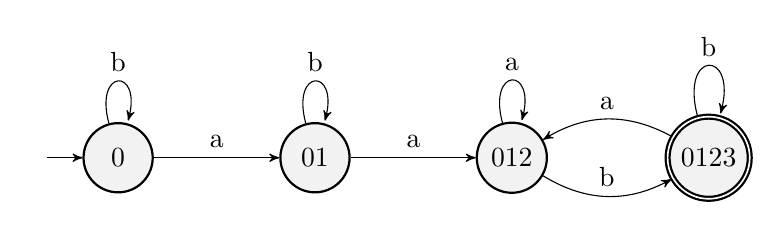
\begin{tikzpicture}
		\node[state, initial] (0) {0};
		\node[state, right of=0] (01) {01};
		\node[state, right of=01] (012) {012};
		\node[state, right of=012, accepting] (0123) {0123};
		\draw (0) edge[above] node {a} (01)
        (0) edge[loop above] node {b} (0)
        (01) edge[above] node {a} (012)
        (01) edge[loop above] node {b} (01)
        (012) edge[loop above] node {a} (012)
        (012) edge[above, bend right] node {b} (0123)
        (0123) edge[above, bend right] node {a} (012)
        (0123) edge[loop above] node {b} (0123);
	\end{tikzpicture}
\end{center}

\subsection*{Fig. 3.29}
\begin{center} % ’ht’ tells LaTeX to place the figure ’here’ or at the top of the page
	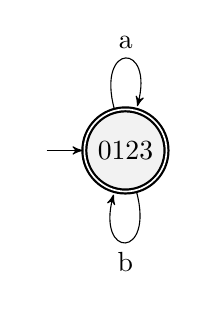
\begin{tikzpicture}
		\node[state, initial, accepting] (0123) {0123};
        \draw (0123) edge[loop above] node{a} (0123)
        (0123) edge[loop below] node{b} (0123);	\end{tikzpicture}
\end{center}

%\begin{center}
%	\includegraphics*[scale=0.21]{0308.jpg}
%\end{center}

\end{document}
